\section{Future Work}
\begin{frame}{Future Work}
  \begin{itemize}
    \item Investigate and interpret the instability of an accelerating flow with non-zero left boundary. See Fig.\ref{fig:accelerating-v-nonzero-bc}
    \item Compare results to analytically solvable problems with similar configuration.
  \end{itemize}

  \begin{figure}[htbp]
    \centering
    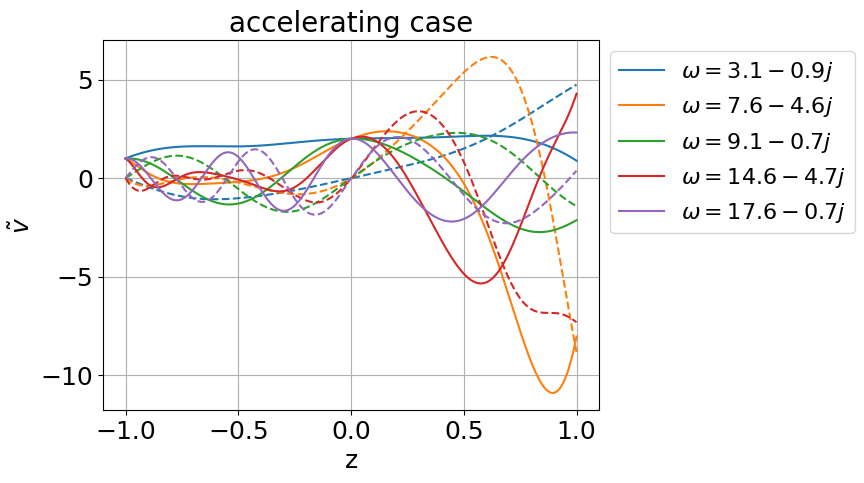
\includegraphics[width=0.6\textwidth]{figures/numerical-experiments/accelerating-v-nonzero-bc}
    \caption{What is the physical interpretation of "non-zero" boundary value? How do we interpret these eigenvalues?}
    \label{fig:accelerating-v-nonzero-bc}
  \end{figure}
\end{frame}
